\section{Red de distribuci�n de agua potable}
Conjunto de elementos enlazados de tal manera que permite suministrar cierta cantidad de agua a una presi�n establecida \cite{Doctoral2012}.

\subsubsection{Caudal}
Cantidad de agua que se mueve a trav�s de un segmento de la red.

\subsection{Componentes f�sicos de una red}
A continuaci�n se define los componentes que conforman una red de agua potable \cite{Rossman2017}, los cuales se aprecian en la Figura \ref{fig:componentesfisicos}:


\begin{figure}[h]
	 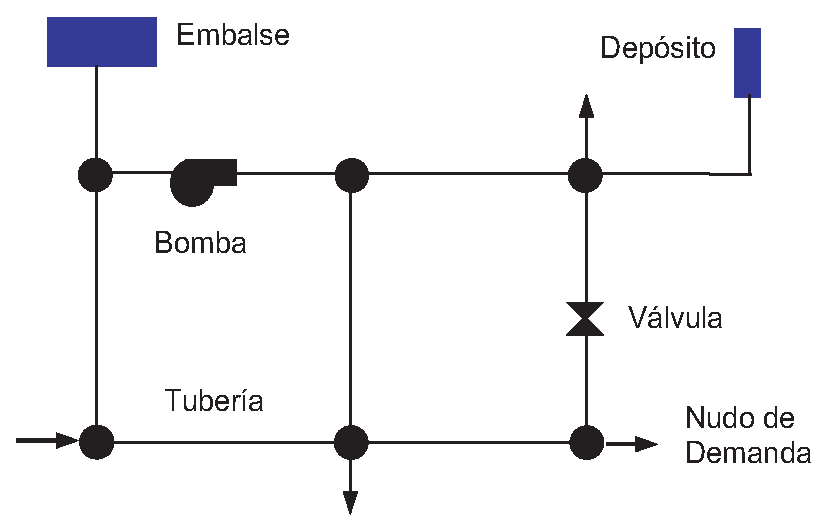
\includegraphics{Capitulo2/assets/componentesfisicosred.eps}
	\centering
	\caption{Componentes f�sicos de un sistema de distribuci�n de agua \cite{Rossman2017}}
	\label{fig:componentesfisicos}
\end{figure}
\subsubsection{Nudos de caudal}

Son los puntos o extremos de una tuber�a, los cuales tambi�n permiten que estas se unan. Estos nudos pueden actuar como nudos de demanda a trav�s de los cuales el flujo abandona la red.

\subsubsection{Embalse}
Es una fuente de alimentaci�n externa.
\subsubsection{Deposito}
Son elementos con la capacidad de almacenar agua.
\subsubsection{Tuber�a}
 Son los elementos a trav�s de los cuales transita el agua de un nudo a otro.
\subsubsection{Bomba}
Elementos que permiten impulsar el liquido con el fin de elevarlo a una posici�n superior.
\subsubsection{V�lvula}
Elementos que limitan la presi�n o el caudal que transita en un punto de la red.
\subsection{Epanet}
Software que permite simular el comportamiento hidr�ulico y la calidad del agua en redes de distribuci�n de aguas compuesta por tuber�as, nodos, bombas, v�lvulas y tanques de almacenamiento \cite{Rossman2017}.  Este software cuenta tambi�n con una librer�a din�mica conocida bajo el nombre de Epanet Programming Toolkit, la cual cuenta con un conjunto de funciones para realizar simulaciones desde diferentes entornos de desarrollo como C, C++, VB, Java, etc \cite{Rossman1999}.